\section{Inbetriebnahme der Turtlebots}
In diesem Teil der Arbeit wird die praktische Umsetzung der Navigationsalgorithmen diskutiert, wofür ROS verwendet wird. Unter ROS werden so genannte Launch-Dateien genutzt, um die beteiligten Pakete zu parametrisieren und zu starten. Typischerweise werden in jedem ROS-Projekt mehrere Launch-Dateien angelegt, die für die jeweiligen Anwendungsfälle ausgelegt sind. In dieser Arbeit werden zwei verschiedene Projekte angelegt. Auf dem Master-PC wird das Projekt \lstinline{EML_Navigation_Master}{} genutzt; auf den Slave-PCs das Projekt \lstinline{EML_Navigation_Slave}{}. Die Projektordner sind jeweils auf den Desktops der PCs zu finden. In dem Master-Projekt werden die vier Launch-Dateien
\begin{itemize}
\item \lstinline{EML_Mapping_Master.launch}{}
\item \lstinline{EML_Navigation_Master.launch}{}
\item \lstinline{EML_Navigation_Robot2_Master.launch}{}
\item \lstinline{EML_Navigation_Robot4_Master.launch}{}
\end{itemize}
genutzt, wobei die erste für die Kartenerstellung, die zweite für die Navigation eines einzelnen Roboters und die beiden letzten für die simultane Navigation der beiden Roboter verwendet werden.

In den Slave-Projekten sind die fünf Launch-Dateien
\begin{itemize}
\item \lstinline{EML_Hardware_Init_Slave.launch}{}
\item \lstinline{EML_Mapping_Slave.launch}{}
\item \lstinline{EML_Navigation_Slave.launch}{}
\item \lstinline{EML_Navigation_Robot2_Slave.launch}{}
\item \lstinline{EML_Navigation_Robot4_Slave.launch}{}
\end{itemize}
zu finden. Die Erste führt die Initialiserung der vorhandenen Hardware durch. Die vier weiteren Dateien stellen das Pendant zu den oben beschriebenen Master-Dateien dar.

\newpage
\subsection{Fernsteuerung eines Turtlebots}
Im aller ersten Schritt werden die beiden Roboter in Betrieb genommen, wofür die Fernsteuerung der beiden Geräte als Demonstration dienen soll. Auf den Slaves wird dafür die Launch-Datei \lstinline{EML_Hardware_Init_Slave.launch}{} angelegt, die die vorhandene Hardware initialisiert, sodass der Roboter über die entsprechenden ROS-Nachrichten bewegt werden kann.
\begin{lstlisting}[caption={EML\_Hardware\_Init\_Slave.launch},captionpos=b]
<launch>
	<!-- Basis-Initialisierung -->
	<include file="$(find turtlebot_bringup)/ ...
			launch/minimal.launch"/>
	
	<!-- Initialisierung des SICK-TIM551 -->
	<param name="robot_description" command="$(find xacro)/ ...
			xacro.py '$(find sick_tim)/urdf/example.urdf.xacro'"/>
	<include file="$(find turtlebot_chor_navigation)/launch/ ...
			include/sick_tim551_2050001_timefix.launch"/>
</launch>
\end{lstlisting}
In der Launch-Datei wrid zunächst eine Basisinitialisierung durchgeführt, wofür die Datei \lstinline{minimal.launch}{} aus dem offiziellem ROS-Packet \lstinline{turtlebot_bringup}{}\cite{WikiTurtlebotBringup} inkludiert wird. Als Zweites wird mithilfe einer der Launch-Datei \lstinline{sick_tim_551_2050001_} \lstinline{timefix.launch}{} aus dem Vorgängerprojekt \cite{Turtleboys} der SICK-Laserscanner initialisiert.

Um den Turtelbot über den Master-PC zu steuern, wird die Launch-Datei auf dem Slave ausgeführt.
\begin{lstlisting}[language=bash]
roslaunch EML_Navigation_Slave EML_Hardware_Init_Slave.launch
\end{lstlisting}
Die Eingabe der Steuerbefehle erfolgt auf dem Master-PC, wofür auf das Paket \lstinline{turtle}{} \lstinline{bot_teleop}{} \cite{WikiTurtlebotTeleop} zurückgegriffen wird. Zum Start wird der Befehl
\begin{lstlisting}
roslaunch turtlebot_teleop keyboard_teleop.launch
\end{lstlisting}
auf dem Master-PC ausgeführt. Daraufhin kann der Roboter mittels der Tastatur bewegt werden.

\newpage
\subsection{Aufzeichnung einer Karte}
Im nächsten Schritt wird die Kartographierung der Umgebung betrachtet, wobei die Ergebnisse der Vorgängerarbeit \cite[S. 47, ff]{Turtleboys} verwendet werden können. Auf Slave-Seite wird die Launch-Datei \lstinline{EML_Mapping_Slave.launch}{} verwendet, in zunächst die bereits angesprochene Datei zur Hardware-Initialisierung inkludiert wird. Im Anschluss werden die Launch-Dateien für die Kartenaufzeichnung des Pakets \lstinline{hector_mapping}{} \cite{WikiHector} eingebunden.
\begin{lstlisting}[caption={EML\_Mapping\_Slave.launch},captionpos=b]
<launch>
	<!-- Hardware-Initialisierung -->
	<include file="$(find EML_Navigation_Slave)/launch/ ... 
			EML_Hardware_Init_Slave.launch" />

	<!-- Hector-Mapping -->
	<node name="hector_mapping" pkg="hector_mapping" ...
			type="hector_mapping" output="screen">
        	<param name="base_frame" value="base_link"/>
        	<param name="odom_frame" value="base_link"/>
	        <param name="map_resolution" value="0.05"/>
	        <param name="map_size" value="2048"/>
	        <param name="map_start_x" value="0.5"/>
        	<param name="map_start_y" value="0.5"/>
	        <param name="map_update_distance_thresh" value="0.4"/>
	        <param name="map_update_angle_thresh" value="0.02"/>
	        <param name="map_pub_period" value="0.05"/>
	        <param name="map_multi_res_levels" value="2"/>
	        <param name="update_factor_free" value="0.4"/>
	        <param name="update_factor_occupied" value="0.9"/>
	        <param name="laser_min_dist" value="0.4"/>
	        <param name="laser_max_dist" value="10"/>
	        <param name="laser_z_min_value" value="-1.0"/>
	        <param name="laser_z_max_value" value="1.0"/>
	        <param name="pub_map_odom_transform" value="true"/>
	        <param name="output_timing" value="false"/>
	        <param name="scan_subscriber_queue_size" value="1"/>
	        <param name="pub_map_scanmatch_transform" ...
	        		value="true"/>
	        <param name="pub_map_scanmatch_transform" ...
	        		value="true"/>
	        <param name="tf_map_scanmatch_transform_ ...
	        		frame_name" value="scanmatcher_frame"/>
	    </node>
    <include file="$(find hector_geotiff)/launch/ ...
    		geotiff_mapper.launch"> </include>
    <node pkg="tf" type="static_transform_publisher" ...
    		name="map_nav_broadcaster" args="0.12 0 0 0 0 0 ...
    		base_link laser 100"/>
</launch>
\end{lstlisting}
Auf dem Master wird die Launch-Datei \lstinline{EML_Mapping_Master.launch}{} verwendet, die inhaltlich ebenfalls aus dem Vorgängerprojekt \cite{Turtleboys} übernommen ist. In der Datei wird lediglich \lstinline{Rviz}{} gestartet, um die Ergebnisse der Kartenerstellung zu visualisieren.
\begin{lstlisting}[caption={EML\_Mapping\_Master.launch},captionpos=b]
<launch>
	<!-- Starte Rviz, um Karte anzuzeigen. -->
	<param name="robot_description" command="$(find xacro)/ ...
			xacro.py '$(find sick_tim)/urdf/example.urdf.xacro'" />
	<node pkg="rviz" type="rviz" name="rviz" args="-d $(find ...
			turtlebot_chor_navigation)/rviz_cfg/rviz_sick.rviz"/>
</launch>
\end{lstlisting}
Neben den beiden Launch-Dateien muss wieder eine Anwendung zur Steuerung des Turtlebots gestartet werden. Außerdem muss am Ende der Kartenaufzeichnung die Applikation \lstinline{map_server}{} ausgeführt werden, um die Karte abzuspeichern. Es ergibt sich die folgende Anleitung für die Kartenaufzeichnung. Die einzelnen Schritten sind in \cite[S. 47 ff]{Turtleboys} ausführlich beschrieben.
\begin{lstlisting}[caption={Anleitung zur Kartenaufzeichnung},captionpos=b]
[M] roscore
[S] roslaunch EML_Navigation_Slave  EML_Mapping_Slave.launch
[M] roslaunch EML_Navigation_Master EMl_Mapping_Master.launch
[M] roslaunch turtelbot_teleop keyboard_teleop.launch
[M] rosrun map_server map_saver
\end{lstlisting}

\newpage
\subsection{Navigation eines einzelnen Roboters}
Nachdem eine Karte der Umgebung erstellt wurde, kann diese für die Navigation eines Roboters herangezogen werden. Auf dem Slave wurde dafür die Launch-Datei \lstinline{EML_Navigation_Slave.launch}{} angelegt, die lediglich eine Hardware-Initialisierung durchführt.
\begin{lstlisting}[caption={EML\_Navigation\_Slave.launch},captionpos=b]
<launch>
	<include file="$(find EML_Navigation_Slave)/launch/ ...
			EML_Hardware_Init_Slave.launch" />
</launch>
\end{lstlisting}
Auf dem Master wird die Launch-Datei \lstinline{EML_Navigation_Master.launch}{} verwendet, in der sämtliche Algorithmen der Navigation parametrisiert und gestartet werden.
\begin{lstlisting}[caption={EML\_Navigation\_Master.launch},captionpos=b]
<launch>
	<!-- Map-Server -->
	<arg name="map_file" default="$(find EML_Navigation_Master)...
			/maps/test_map.yaml"/>
	<node name="map_server" pkg="map_server" type="map_server" ...
			args="$(arg map_file)"/>
	<!-- AMC-Localization -->
	<arg name="3d_sensor" default="$(env TURTLEBOT_3D_SENSOR)"/>
	<arg name="initial_pose_x" default="0.0"/>
	<arg name="initial_pose_y" default="0.0"/>
	<arg name="initial_pose_a" default="0.0"/>
	<arg name="custom_amcl_launch_file" default="$(find ...
			turtlebot_navigation)/launch/includes/amcl/$...
			(arg 3d_sensor)_amcl.launch.xml"/>
	<include file="$(arg custom_amcl_launch_file)">
		<arg name="initial_pose_x" ...
				value="$(arg initial_pose_x)"/>
		<arg name="initial_pose_y" ...
				value="$(arg initial_pose_y)"/>
		<arg name="initial_pose_a" ...
				value="$(arg initial_pose_a)"/>
		<arg name="odom_frame_id" value="odom"/>
		<arg name="base_frame_id" value="base_footprint"/>
		<arg name="global_frame_id" value="map"/>
		<arg name="use_map_topic" value="true"/>
	</include>
	<!-- Static Transform from base_footprint to base_link -->
	<node pkg="tf" type="static_transform_publisher" ...
			name="base_link_footprint_tf_broadcaster"...
			args="0 0 .5 0 0 0 1 base_footprint base_link 100"/>
	<!-- Rviz -->
	<node name="rviz" pkg="rviz" type="rviz" args="-d ...
			$(find turtlebot_rviz_launchers)/rviz/navigation.rviz"/>
	<!-- move_base -->
	<include file="$(find EML_Navigation_Master) ...
			/launch/include/eml_move_base.launch"/>
</launch>
\end{lstlisting}

In der Datei wird zunächst die AMC-Lokalisierung gestartet, wofür die Standardparameter des ROS-Pakets \lstinline{amcl} \cite{WikiAMCL} genutzt werden. Des Weiteren wird \lstinline{Rviz}{} gestartet, womit die Karte, Position des Roboters sowie die Zielposition graphisch dargestellt werden. Als Konfiguration dient die Datei \lstinline{navigation.rviz}{}, die in dem ROS-Paket \lstinline{turtlebot_rviz_launchers} \cite{WikiRVIZLaunchers} enthalten ist. Zuletzt wird das Paket \lstinline{move_base} \cite{WikiMoveBase} gestartet, in dem die letztendliche Navigation berechnet wird. Als Konfigurationsdatei dient \lstinline{eml_move_base.launch}{}, welche die \lstinline{move_base}{}-Instanz parametrisiert.
\begin{lstlisting}[caption={eml\_move\_base.launch},captionpos=b]
<launch>
	<include file="$(find turtlebot_navigation)/launch/ ...
			includes/velocity_smoother.launch.xml"/>
	<include file="$(find turtlebot_navigation)/launch/ ...
			includes/safety_controller.launch.xml"/>
  
	<arg name="odom_frame_id"   default="odom"/>
	<arg name="base_frame_id"   default="base_footprint"/>
	<arg name="global_frame_id" default="map"/>
	<arg name="odom_topic" default="odom" />
	<arg name="laser_topic" default="scan" />
	<arg name="custom_param_file" default="$(find ...
			turtlebot_navigation)/param/dummy.yaml"/>

	<node pkg="move_base" type="move_base" respawn="false" ...
			name="move_base" output="screen">
	<rosparam file="$(find EML_Navigation_Master)/param/ ...
			eml_costmap_common_params.yaml" command="load" ...
			ns="global_costmap" />
	<rosparam file="$(find EML_Navigation_Master)/ ...
			param/eml_costmap_common_params.yaml"    ...
			command="load" ns="local_costmap" />   
	<rosparam file="$(find turtlebot_navigation)/param/ ...
			local_costmap_params.yaml" command="load" />   
	<rosparam file="$(find turtlebot_navigation)/param/ ...
			global_costmap_params.yaml" command="load" />
	<rosparam file="$(find EML_Navigation_Master)/param/...
			eml_dwa_local_planner_params.yaml" command="load" />
	<rosparam file="$(find turtlebot_navigation)/param/...
			move_base_params.yaml" command="load" />
	<rosparam file="$(find turtlebot_navigation)/param/...
			global_planner_params.yaml" command="load" />
	<rosparam file="$(find turtlebot_navigation)/param/...
			navfn_global_planner_params.yaml" command="load" />
	    
	<!-- reset frame_id parameters using user input data -->
	<param name="global_costmap/global_frame" ...
			value="$(arg global_frame_id)"/>
	<param name="global_costmap/robot_base_frame" ...
			value="$(arg base_frame_id)"/>
    <param name="local_costmap/global_frame" ...
    		value="$(arg odom_frame_id)"/>
    <param name="local_costmap/robot_base_frame" ...
    		value="$(arg base_frame_id)"/>
    <param name="DWAPlannerROS/global_frame_id" ...
    		value="$(arg odom_frame_id)"/>

    <remap from="cmd_vel" ...
    		to="navigation_velocity_smoother/raw_cmd_vel"/>
    <remap from="odom" to="$(arg odom_topic)"/>
    <remap from="scan" to="$(arg laser_topic)"/>
  </node>
</launch>
\end{lstlisting}
Allerdings wurden hier lediglich Standardparameter verwendet, die aus dem Demonstrationsbeispiel des \lstinline{move_base}{} \cite{WikiMoveBase} Paket stammen. In der Konfigurationsdatei werden wiederum Parameterdateien geladen, wobei die meisten aus dem Paket \lstinline{turtlebot_} \lstinline{navigation}{} \cite{WikiTBNavigation} stammen. Für Versuchszwecke wurden in dieser Konfiguration Parameterdateien für die Kostenkarte und den lokalen Planer durch eigene Implementierungen ersetzt. Dadurch können Änderung an den Parametersätzen vorgenommen werden.

Um die Navigation auszuführen, muss die beiden Launch-Dateien auf Slave und Master ausgeführt werden. Allerdings ist anzumerken, dass nach dem Neustart der Systeme deren Uhrzeiten synchronisiert werden müssen, wofür der Befehl \lstinline{ntpdate}{} herangezogen wird.
\begin{lstlisting}[caption={Anleitung Navigation eines Roboters},captionpos=b]
[S] sudo ntpdate 192.168.0.100
[M] soscore
[S] roslaunch EML_Navigation_Slave  EML_Navigation_Slave.launch
[M] roslaunch EML_Navigation_Master EML_Navigation_Master.launch
\end{lstlisting}

\subsection{Navigation mehrerer Roboter}
Das Endziel dieser Arbeit besteht darin, dass zwei Roboter sich simultan durch einen Raum bewegen. Dabei kommunizieren beide Geräte über dasselbe ROS-Netzwerk, weshalb Namenskonflikte bei der Nachrichtenkommunikation auftreten. Beispielsweise wird die Topic \lstinline{scan}{}, welche die Laserscandaten enthält, von beiden Robotern veröffentlicht, wenn die obige Launch-Datei auf beiden Slave-PCs ausgeführt wird. So kann bei der Auswertung der Sensordaten nicht mehr zwischen den beiden Robotern differenziert werden.

Eine mögliche Lösung stellen die \lstinline{group}{}-Tags \cite{WikiGroup} unter ROS dar, mit denen jeder ROS-Node ein Namensraum zugeordnet werden kann. Als erstes Beispiel dient die Launch-Datei \lstinline{EML_NS_Hardware_Init_Slave.launch}{} auf dem Slave, welche die Hardware unter der Verwendung eines Namensraum initialisiert.
\begin{lstlisting}[caption={EML\_NS\_Hardware\_Init\_Slave.launch},captionpos=b]
<launch>
        <arg name="namespace" default="Robot"/>
        <group ns="$(arg namespace)">
                <!-- Basis-Initialisierung -->
                <include file="$(find turtlebot_bringup)/ ...
                		launch/minimal.launch"/>

                <!-- Initialisierung des SICK-TIM551 -->
                <param name="robot_description" command= ...
                		"$(find xacro)/xacro.py '$(find  ...
                		sick_tim)/urdf/example.urdf.xacro'"/>
                <include file="$(find turtlebot_chor_ ...
                		navigation)/launch/include/   ...
                		sick_tim551_2050001_timefix.launch"/>
        </group>
</launch>
\end{lstlisting}
Die Launch-Datei kann mit dem zusätzlichen Argument \lstinline{namespace}{} gestartet werden, wodurch der Namensraum der Knoten festgelegt wird. So führt der Befehl
\begin{lstlisting}
roslaunch EML_Navigation_Slave  ...
		EML_NS_Hardware_Init_Slave.launch namespace:="R4"
\end{lstlisting}
dazu, dass jeder Topic der Präfix \lstinline{/R4/}{} hinzugefügt wird, wodurch eine klare Zuordnung zwischen Nachricht und Roboter erfolgt. Auf dem zweiten Roboter muss lediglich der \lstinline{namespace}{}-Parameter angepasst werden.

Ebenso wird auf dem Master die Launch-Datei \lstinline{EML_NS_Teleop_Master.launch}{} angelegt, womit die Fernsteuerung der Roboter unter Namensräumen erfolgen kann.
\begin{lstlisting}[caption={EML\_NS\_Teleop\_Master.launch},captionpos=b]
<launch>
        <arg name="namespace" default="Robot"/>
        <group ns="$(arg namespace)">
                <include file="$(find turtlebot_teleop)/ ...
                		launch/keyboard_teleop.launch"/>
        </group>
</launch>
\end{lstlisting}
Prinzipiell sollte es möglich sein, die Navigation nach demselben Ansatz mit einem Namensraum zu versehen und dadurch die beiden Roboter zu entkoppeln. Hierfür wird die Slave-Datei \lstinline{EML_NS_Navigation_Slave.launch}{} angelegt.
\begin{lstlisting}[caption={EML\_NS\_Navigation\_Slave.launch},captionpos=b]
<launch>
	<arg name="namespace" default="Robot"/>
    <group ns="$(arg namespace)">
    	<!-- Map-Server -->
        <arg name="map_file" default="$(find EML_Navigation_ ...
        	Master)/maps/test_map.yaml"/>
        <node name="map_server" pkg="map_server" ...
        	type="map_server" args="$(arg map_file)"/>

		<!-- AMC-Localization -->
        <arg name="3d_sensor" default="$ ...
        	(env TURTLEBOT_3D_SENSOR)"/>
        <arg name="initial_pose_x" default="0.0"/>
        <arg name="initial_pose_y" default="0.0"/>
        <arg name="initial_pose_a" default="0.0"/>
        <arg name="custom_amcl_launch_file" ...
        	default="$(find turtlebot_navigation)/launch/ ...
        	includes/amcl/$(arg 3d_sensor)_amcl.launch.xml"/>

        <include file="$(arg custom_amcl_launch_file)">
        <arg name="initial_pose_x" value= ...
        	"$(arg initial_pose_x)"/>
        <arg name="initial_pose_y" value= ...
        	"$(arg initial_pose_y)"/>
        <arg name="initial_pose_a" value= ...
        	"$(arg initial_pose_a)"/>
        <arg name="odom_frame_id" value="odom"/>
        <arg name="base_frame_id" value="base_footprint"/>
        <arg name="global_frame_id" value="map"/>
        <!-- arg name="scan_topic" value= ...
        	"$(arg namespace)/scan"/-->
        <!-- param name="tf_prefix" value=...
        	"$(arg namespace)"/-->
        <arg name="use_map_topic" value="true"/>
        </include>

		<!-- Static Transform from base_footprint to base_link -->
        <node pkg="tf" type="static_transform_publisher" ...
        	name="base_link_footprint_tf_broadcaster"    ...
        	args="0 0 .5 0 0 0 1 base_footprint base_link 100"/>

        <!-- Rviz -->
        <node name="rviz" pkg="rviz" type="rviz" args="-d ...
        	$(find turtlebot_rviz_launchers)/ ...
        	rviz/navigation.rviz"/>

        <!-- move_base -->
        <include file="$(find EML_Navigation_Master)/launch/...
        	include/eml_move_base.launch"/>
	</group>
</launch>
\end{lstlisting}
An dieser Stelle entsteht das Problem, dass in der \lstinline{Rviz}{}-Konfiguration festgelegt wird, unter welchen Namen die relevanten Nachrichten veröffentlicht werden. Daraus folgt, dass ein Weg gefunden werden muss, die \lstinline{Rviz}{}-Konfiguration ebenfalls mit einem Namensraum zu parametrisieren.
Diese Problematik kann gelöst werden, indem über die Benutzeroberfläche die fehlende Präfixe nachträglich eingefügt werden. Somit ist es möglich \lstinline{Rviz}{} an beliebige Namensräume anzupassen. Aus praktikablen Gründen bietet es sich an, die Konfigurationen zu speichern und nach Programmstart manuell zu laden, um den Aufwand einer manuellen Rekonfiguration zu ersparen.

Als zweites Problem sind die \lstinline{tf}{}-Transformationen zu nennen, bei denen ebenfalls Namenskonflikte entstehen. ROS verwendet einen so genannten Transformation-Tree bzw. \lstinline{tf}{}-Tree, um die Position von Objekten darzustellen. Bei einer Transformation - kurz \lstinline{tf}{} - handelt es sich um eine Abbildung zwischen zwei Bezugssystemen, die im Kontex von ROS als \lstinline{frames}{} bezeichnet werden. Für gewöhnlich fungiert die Karte als Intertialsystem bzw. \lstinline{fixed frame}{}. Eine Transformation gibt dann den Zusammenhang zwischen den Systemen \lstinline{map}{} und \lstinline{robot}{} wieder, wodurch die Position des Roboters festgelegt wird. Offensichtlich übernimmt diese Aufgabe die AMC-Lokalisierung. An dieser Stelle treten wieder dieselben Namenskonflikte wie bei den ROS-Nachrichten auf. Jeder Roboter benötigt einen Transformationsbaum, der von dem des anderen Roboters entkoppelt ist.
\begin{figure}[!ht]
\centering
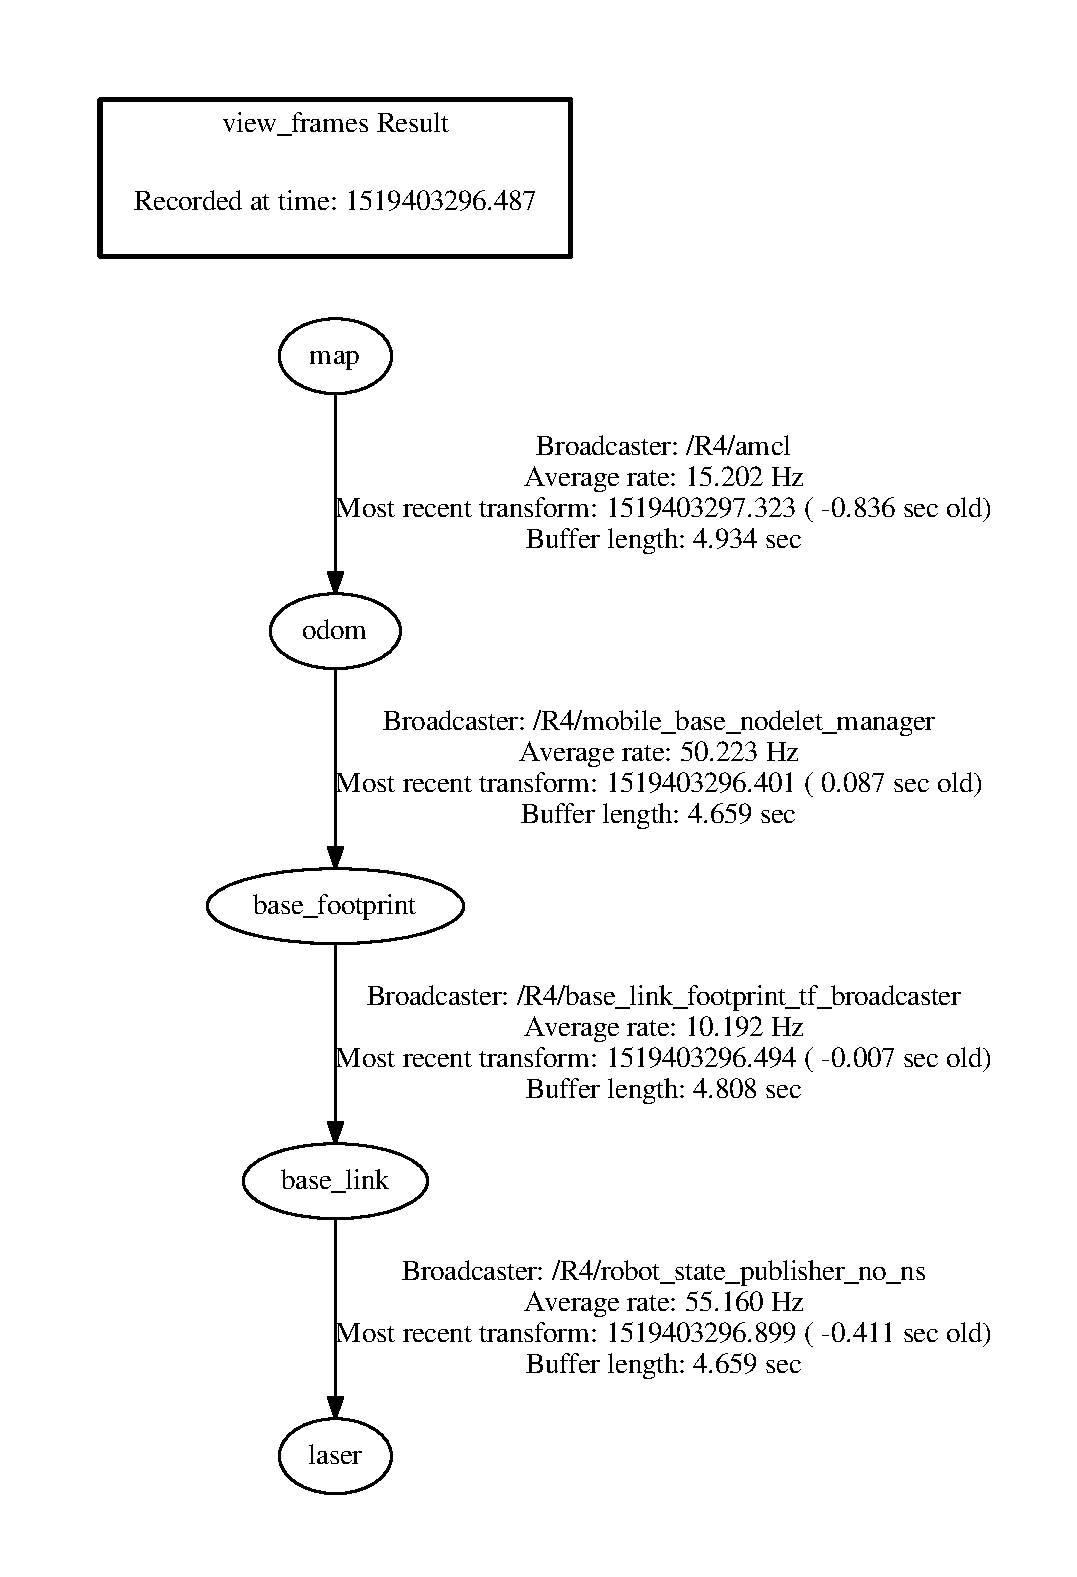
\includegraphics[width=0.4\linewidth, trim={3.5cm 1cm 1cm 5cm},clip]{img/TF_Tree_no_NS.pdf}
\caption{Transformationsbaum von Roboter 4}
\end{figure}
An dieser Stelle sei auf das ROS-Werkzeug \lstinline{tf}{} hingewiesen, das es ermöglicht mittels dem Befehl
\begin{lstlisting}
rosrun tf view_frames
\end{lstlisting}
Grafiken wie die obige zu generieren, wodurch die Fehlerfindung erleichtert wird. In dem aktuellen Transformationsbaum wird zuerst von \lstinline{map}{} nach \lstinline{odom}{} transformiert, wofür der AMCL-Knoten verantwortlich ist. Anschließend veröffentlicht der Knoten \lstinline{mobile_base_nodelet_manager}{} eine Transformation von \lstinline{odom}{} zu \lstinline{base_footprint}{}. Von \lstinline{base_footprint}{} wird wiederum in \lstinline{base_link}{} überführt. Veröffentlicht wird diese Transformation von \lstinline{base_link_footprint_tf_broadcaster}{}. Zuletzt erfolgt die Transformation von \lstinline{base_link}{} zu \lstinline{laser}{}, wofür der Knoten \lstinline{robot_state_publisher} \lstinline{_no_ns}{} zuständig ist. In dem Bezugssystem \lstinline{laser}{} werden die Daten des Laserscanners interpretiert. Bei \lstinline{base_footprint}{} und \lstinline{base_link}{} handelt es sich jeweils um körperfeste Bezugssysteme des Roboters, deren relative Ausrichtung zueinander konstant ist.

Die Knoten \lstinline{base_link_footprint_tf_broadcaster}{} und \lstinline{robot_state_}{}\linebreak  \lstinline{publisher_no_ns}{} werden jeweils über das Slave-Skript gestartet; \lstinline{mobile_base_}{} \lstinline{nodelet_manager}{} und \lstinline{amcl}{} von der Master-Datei aus.

Ein Ansatz, um die Namenskonflikte aufzulösen, besteht darin, den Parameter \lstinline{tf_prefix}{} zu nutzen, womit ähnlich zum \lstinline{group}{}-Tag Präfixe an die Bezugssysteme der Roboter angefügt werden können. Dieser Ansatz wird mittel der Launch-Datei \lstinline{EML_NS_TF_Hardware_Init_Slave.launch}{} verfolgt.
\begin{lstlisting}[caption={EML\_NS\_TF\_Hardware\_Init\_Slave.launch},captionpos=b]
<launch>
	<arg name="namespace" default="Robot"/>
	<group ns="$(arg namespace)">
		<!-- Basis-Initialisierung -->
		<include file="$(find EML_Navigation_Slave)/launch/ ...
				include/EML_minimal.launch">
			<arg name="namespace" value="$(arg namespace)"/>
		</include>
	
		<!-- Initialisierung des SICK-TIM551 -->
		<param name="robot_description" command="$(find xacro)/ ...
			xacro.py '$(find sick_tim)/urdf/example.urdf.xacro'"/>
		<include file="$(find turtlebot_chor_navigation)/...
			launch/include/sick_tim551_2050001_timefix.launch"/>
	</group>
</launch>

\end{lstlisting}
Der primäre Unterschied zu der vorherigen Variante besteht darin, dass die Standarddatei \lstinline{minimal.launch}{} aus dem \lstinline{turtlebot_bringup}{}-Paket durch die Datei \lstinline{EML_minimal.launch}{} ersetzt wurde. Hierbei handelt es sich um eine Kopie der Ausgangsdatei, die um den Namensraumparameter ergänzt wurde, der den jeweiligen ROS-Knoten beim Start übergeben wird. Im relevant Teil von \lstinline{EML_minimal.launch}{} werden drei weitere Launch-Dateien inkludiert, die wiederum durch angepasste Kopien ersetzt werden.
\begin{lstlisting}[caption={Ausschnitt aus EML\_minimal.launch},captionpos=b]
 <arg name="namespace"         default="Robot"/>

  <param name="/use_sim_time" value="$(arg simulation)"/>

  <include file="$(find EML_Navigation_Slave)/launch/ ...
  		include/EML_robot.launch.xml">
    <arg name="stacks" value="$(arg stacks)" />
    <arg name="3d_sensor" value="$(arg 3d_sensor)" />
    <arg name="namespace" value="$(arg namespace)" />
  </include>
  <include file="$(find EML_Navigation_Slave)/launch/ ...
  		include/EML_mobile_base.launch.xml">
    <arg name="serialport" value="$(arg serialport)" />
    <arg name="namespace"  value="$(arg namespace)" />
  </include>
  <include file="$(find EML_Navigation_Slave)/launch/ ...
  		include/EML_netbook.launch.xml">
    <arg name="battery" value="$(arg battery)" />
    <arg name="namespace" value="$(arg namespace)" />
  </include>
\end{lstlisting}
Die drei Dateien \lstinline{EML_robot.launch.xml}{}, \lstinline{EML_mobile_base.launch.xml}{} und \lstinline{EML}{} \lstinline{_netbook.launch.xml}{} sind wiederum angepasste Kopien der Dateien \linebreak \lstinline{robot.launch.xml}{}, \lstinline{mobile_base.launch.xml}{} und \lstinline{netbook.launch.xml}{}, die ebenfalls aus dem Paket \lstinline{turtlebot_bringup}{} entnommen sind. 

Die Hauptproblematik entsteht in der Datei \lstinline{EML_mobile_base.launch.xml}{}, in der die Node \lstinline{mobile_base_nodelet_manager}{} mit den folgenden Zeile gestartet wird.
\begin{lstlisting}[caption={Ausschnitt aus EML\_mobile\_base.launch.xml},captionpos=b]
<node pkg="nodelet" type="nodelet" name="mobile_base_ ...
		nodelet_manager" args="manager">
	<param name="tf_prefix" value="R4" />
</node>
\end{lstlisting}
In diesem Beispiel wird der Parameter \lstinline{tf_prefix}{} auf den fixen Wert R4 gesetzt. Die korrekte Ausführung der Parametrisierung wurde mithilfe des ROS-Befehls
\begin{lstlisting}
rosparam get mobile_base_nodelet_manager/tf_prefix
\end{lstlisting}
geprüft, mit dem Ergebnis, dass der Präfix erfolgreich gesetzt wurde. Allerdings zeigt der Transformationsbaum, dass die ROS-Node den Präfix bei der Transformation nicht verwendet.
\begin{figure}[!ht]
\centering
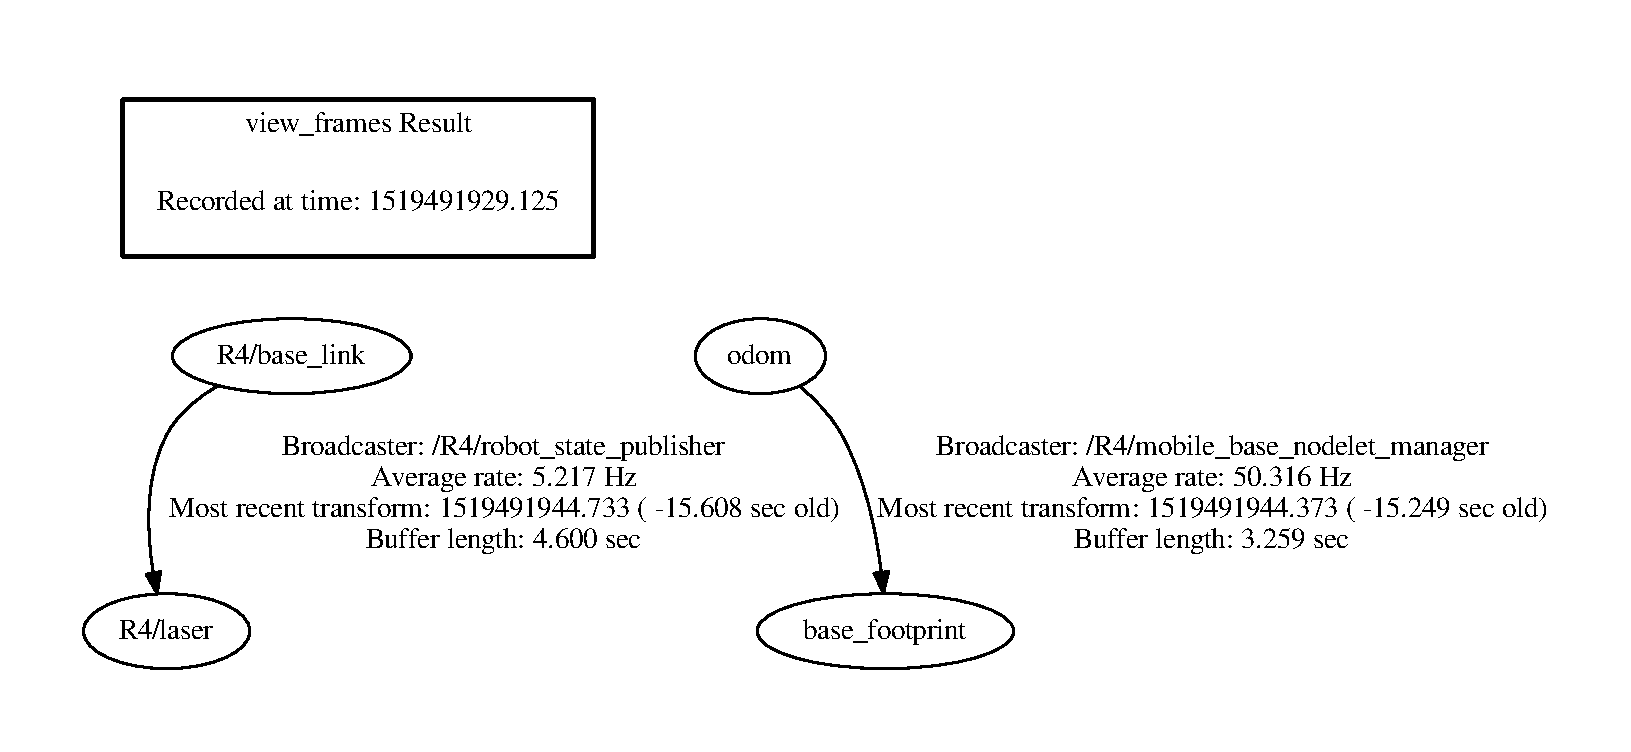
\includegraphics[width=0.8\linewidth, trim={1cm, 1cm, 1cm, 5cm}, clip]{img/TF_Tree_TF_Prefix.pdf}
\caption{Transformationsbaum nach gesetztem Transformationspräfix}
\end{figure}
Das Setzen des Präfixparameter bei dem Knoten \lstinline{robot_state_publisher}{} funktioniert, wie auch in der obigen Abbildung ersichtlich wird, wie erwartet. Insofern handelt es sich um kein prinzipielles Problem des \lstinline{tf_prefix}{}-Parameter. 

Das hier beschriebene Problem macht es zu dem aktuellen Zeitpunkt unmöglich zwei Roboter parallel in Betrieb zu nehmen.